\chapter{Introduction}

\section{Research Background}
Decentralization and sustainable resource sharing are key drivers for success in today’s globalized economy. From craftsmanship to Agile and Intelligent Manufacturing, production has become increasingly complex, depending upon new technological developments and advances in Information and Communication Technologies in response to changes in local and global markets \parencite{model_information_2012}. Moreover, this context and market trends such as mass customization pose new challenges to industries and researchers. The process of sharing resources and assets efficiently on a global scale requires high interoperability, flexibility, and agility in manufacturing systems to respond to rapid changes. Therefore, the rapid evolution of markets and advances in key enabling technologies have introduced the distributed manufacturing paradigm. This paradigm aims to share geographically scattered manufacturing resources and capabilities and already profoundly impact current systems.\\
While the introduction of state-of-the-art technologies presents positive benefits for manufacturing enterprises over competitors, new issues in implementing these network technologies that affect production occur within the manufacturing industry. Most of these issues involve sharing manufacturing resources, where these resources, centralized into a central network, are not distributed efficiently through the platform due to a lack of global coordination in manufacturing services management in the network. And, secondly, the inability to access the independent manufacturing complex resources (equipment) in the manufacturing network due to complications in transferring hardware resources into the network \parencite{laili_study_2012}\parencite{xu_cloud_2012}.\\
Much of the shift towards new paradigms, indeed, is driven by the emergence of Big Data, and the issues connected to the ways by which industrial operations collect, manage and interpret their data remain prevalent\parencite{chen_data_2015}. Considerations about Big Data and the treatment of large datasets are an intrinsic challenge of each system operating in an Industry 4.0 scenario. Traditional statistical processing methods are often useless due to the complexity and the sheer size of large datasets. Current implementations have demonstrated adaptive scheduling, real-time modelling of processes, and Decision Support Systems used to refine processes and component design \parencite{oliff_towards_2017}. For the optimization of issues within the context of production and logistics, a typical aim is gaining quantitative improvements, which also correspond to an increase in resource efficiency \parencite{hauder_optimization_2017}. Sometimes new manufacturing models arise as such a situation leads to increasing adoption of new production technologies. The challenge with distributed production is to implement communication and integration technologies that reduce the coordination effort and provide a focused platform \parencite{khajavi_additive_2014}.\\
Building innovative models around the notion of being “globally virtual, locally physical” calls for a service-dominant logic of distributed resources in which reusable services models, shaped according to the concept of Manufacturing as a Service, represent homogeneous production processes \parencite{kayabay_wip_2018}. Therefore, the ongoing servitization process in the manufacturing industry is progressively shifting the view of traditional resources as a set of services and solutions that supplement companies’ traditional offerings consumed on an ad-hoc basis \parencite{bo-hu_cloud_2010}. As a result, enterprises increase their capability to provide manufacturing services and offer more extensive and more complex jobs. Moreover, Cloud Manufacturing, with the proper implementation,presents the capability to transform and restructure manufacturing systems and move the entire industry from production-oriented manufacturing to service-oriented manufacturing \parencite{xu_cloud_2012}. Cloud Manufacturing can also be a significant factor to reduce costs, maximize productivity, reduce time to market, and increase business agility and innovation \parencite{ren_cloud_2017}, as well as facilitating the whole life cycle of manufacturing, providing safe, reliable, high-quality, cheap, and on-demand manufacturing services \parencite{zhang_cloud_2014}.\\
Other potential benefits from the introduction of Cloud Manufacturing are the following \parencite{ren_cloud_2017}:
\begin{enumerate}
    \item Virtual access to homogenous and interoperable manufacturing services over the cloud, reducing the need to invest, develop, maintain, and manage hardware and software manufacturing resources.
    \item Higher utilization rates of manufacturing resources through the promotion of shared pools of resources.
    \item Higher Scalability, encouraging Cloud Manufacturing users to control production capacity to balance the current demand dynamically.
    \item The introduction of novel utility-based cost schemes that assigns costs based on user/provider resources consumptions.
    \item An on-demand approach that endorses users to have ubiquitous access and natural human-computer interaction to manufacturing resources.
\end{enumerate}
Main issues for enabling the transition to cloud manufacturing, as recent research efforts have summarized the main challenges for cloud manufacturing as follows:
\begin{enumerate}
    \item Unclear principles for the protection of the end-user investment. The new business model that comes with cloud manufacturing requires fresh perspectives on the protection of rights.
    \item Difficulty in communication and interaction between departments within the enterprise and among the stakeholders within the supply chain due to different systems with different focuses.
    \item Limited collaboration and interaction between business partners within cloud manufacturing.
    \item Absence of a readily available implementation framework for cloud manufacturing services. Each company has to implement this as a new system.
    \item Difficulty in the deployment of physical resources, such as machines, monitors, and facilities. These issues are mainly due to the unpreparedness of a large portion of resources for the required connectivity.
\end{enumerate}
This research attempts to answer some of these issues. In particular, an attempt to formalize the main founding principles that a Cloud Manufacturing platform should obey (see \autoref{chapter3-sec2}). Moreover, a Multi-Agent Systems architecture for distributed operations is provided to identify the key process parameters for selecting communication approaches within service providers and service demanders. Finally, an implementation framework is depicted in the context of a large Additive Manufacturing Network scenario. The architectural model is used to simulate communications and operations in the scenario, while the implementation model is used to define an optimization algorithm to manage both scheduling and logistics problems using one cycle of negotiation.
\section{Thesis Outline}
This Thesis is divided into five chapters, as shown in Figure \ref{fig:thesis-outline}. Chapter I "\nameref{chapter1}" provides a background and general overview of the research project, followed by an introduction of the research motivation, research scope, research aim,and objectives. The first chapter also outlines the remaining chapters of the Thesis. Chapter II "\nameref{chapter2}" provides reviews of the literature on two main concepts: Cloud Manufacturing and Cloud Manufacturing Architecture. In phase one of the literature review, the focus was on cloud manufacturing and its types, characteristics, and attributes. In phase 2, the focus was on understanding architectures and exploring the role of autonomy and independence of resources in distributed manufacturing systems and their effects in the cloud environment. Phase 2 also identifies the research gap. Chapter III "\nameref{chapter3}" develops a framework to manage autonomous resources in cloud manufacturing. This chapter begins by introducing and explaining the phases of development of the framework. It then explores the process of identifying differences with frameworks available from literature in a detailed comparison. Then, it outlines in-depth platform actors, roles, functionalities, and service management systems through an analysis of main platform factors, dynamics, and governance. Chapter IV "\nameref{chapter4}" presents two implementing models of the proposed architecture. In model 1, the focus was on developing a Multi-Agent Systems architecture for distributed operations in presence of autonomous service providers. In model 2, the focus was on developing an optimization model that combines localization, fragmentation, assignment, and picking issues for a specific job order in a large Additive Manufacturing Network. Chapter V "\nameref{chapter5}" summarizes the results, draws conclusions, and makes recommendations for future work. This chapter presents outcomes, including the research contribution to knowledge, research limitations, and future work. Also, it reveals answers to the research aim and objectives and presents the overall research conclusion.

\begin{figure}[h]
    \centering
    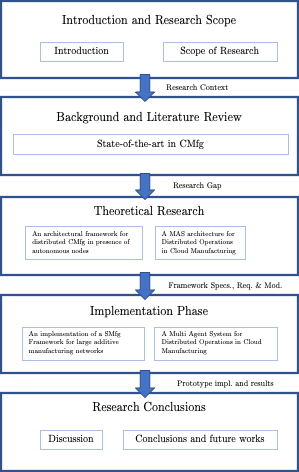
\includegraphics[height=10cm, keepaspectratio]{images/thesis-outline.png}
    \caption{Thesis Outline}
    \label{fig:thesis-outline}
\end{figure}
